\documentclass[12pt]{article}
\usepackage{geometry}                % See geometry.pdf to learn the layout options. There are lots.
\geometry{letterpaper}                   % ... or a4paper or a5paper or ... 
\usepackage{graphicx}
\usepackage{amssymb}
\usepackage{amsthm}
\usepackage{epstopdf}
\usepackage[utf8]{inputenc}
\usepackage[usenames,dvipsnames]{color}
\usepackage[table]{xcolor}
\usepackage{hyperref}
\DeclareGraphicsRule{.tif}{png}{.png}{`convert #1 `dirname #1`/`basename #1 .tif`.png}

\theoremstyle{definition}
\newtheorem{example}{Example}

\newenvironment{explanation}{%
   \setlength{\parindent}{0pt}
   \itshape
   \color{blue}
}{}

\newcommand{\projectname}{FinanceM}
\newcommand{\productname}{Finance application for yout Smartphone}
\newcommand{\projectleader}{C. Tumfart, L. Trimbacher}
\newcommand{\documentstatus}{In process}
%\newcommand{\documentstatus}{Submitted}
%\newcommand{\documentstatus}{Released}
\newcommand{\version}{V. 1.0}

\begin{document}
\begin{titlepage}
\begin{flushright}

\includegraphics[scale=.5]{htlleondinglogo.png}\\
\end{flushright}

\vspace{10em}

\begin{center}
{\Huge Project Proposal} \\[3em]
{\LARGE \productname} \\[3em]
\end{center}

\begin{flushleft}
\begin{tabular}{|l|l|}
\hline
Project Name & \projectname \\ \hline
Project Leader & \projectleader \\ \hline
Document state & \documentstatus \\ \hline
Version & \version \\ \hline
\end{tabular}
\end{flushleft}

\end{titlepage}
\section*{Revisions}
\begin{tabular}{|l|l|l|}
\hline
\cellcolor[gray]{0.5}\textcolor{white}{Date} & \cellcolor[gray]{0.5}\textcolor{white}{Author} & \cellcolor[gray]{0.5}\textcolor{white}{Change} \\ \hline
&C. Tumfart/L. Trimabcher&First version \\ \hline
\end{tabular}
\pagebreak

\tableofcontents
\pagebreak

\section{Introduction}
The FinanceM application should be a helping hand to have an overview about your finances. The user can document his money flow. 
With an userfriendly interface the application makes it much easiert to work understand details even if you are not into technologie or businnes.
After all it should be an application which is easy to handle that helps the user to have a better overview about his in and outgoings.
\pagebreak

\section{Initial Situation}

The pronblem of developing a finance application is that there is a wide range of finance apps but they all got the same problems.
They got all features users could imagine but none got it all.
There is always a lack of features like cashmanagement, connection to the bankaccount, profit/loss etc.

\pagebreak

\section{General Conditions and Constraints}

To run the application smoothly and without technical incidents
the default language is english and easy usable for the user.
Further saving userdata on the device is more secure but with the idea of an ios based application an ICloud backup keeps data in case the mobile phone gets lost, gets damaged etc.
With using PSD2 it is possible to synchronise the application with the users bank account and an realtime connection to get bookings and finance informations
\\

Like in the section above the application only runs on IOS, for storing and data Security reasons. Furthermore PSD2 must be used, outherwise the application hasn't access to the bankaccount of the user.
\pagebreak

\section{Project Objectives and System Concepts}

The objectives of the project which are in the foreground are that 
it is easy for the user to see the informations in a structured way on an different dashboards which either goes depeper in different parts of your finances(outgoings -> food, technical etc.) or 
shows a summary wich is as informativ as possible and as short as needed at the same time which a
The last main objectiv treats that in and outgoings are collected into groups as food, mobility, technical gadgets, etc. 
\\
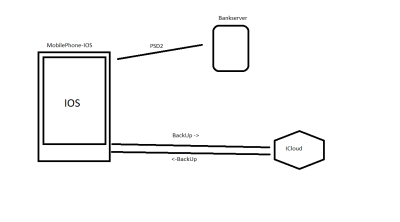
\includegraphics[scale=1.2]{Organisation.png}

The mobile phone will communicate via PSD2 with the bankserver so that the application has access to the incomes and outcomes of the user.
The App will initially only run on ios, because we store the userdata on the mobile phone itself. So someone might think what happens is I lose my phone...
thats the reason we only use ios because you can just download the latest backup of your phone and still have your data.
That will be the better solution for now, because the data will be savely stored on an ICloud server.

\subsection{Organisation}

We got more expirience with using IOS so we decided that the app is going to be IOS based which supports the backup idea through the ICloud service.



\pagebreak
\section{Opportunities and Risks}

The applications opportunities are to revolutionize the market around finance apps
through filling the lack of features by creating a single app that encludes all known and usefull featuers like profit/loss, cashmanagement, direkt connection to the users bankaccount etc. which finance apps should contain. 
\\

Every project got risks which in this case is the big market.
With a market full of different variations of applications its hard to develop a new one and make it a success 
but with the rigth features and a difference between FinanceM with a wide and also deep range of useabilities it is possible to overcome the risks.

\pagebreak
\section{Planning}

Project Leaders and an overview of how much resources we need
\\

Project Leaders: Lukas Trimabcher and Christoph Tumfart
\\

Resources we need:
\\

We need 2 people to do the coding and maybe someone to help us with the graphical part of the user interface. Apart from that we need a license so we can get access to the bank accounts of the users.
And of course another server on which we save the user data.
\\

November 12th:
\\

The project will start. This is where we start to implement the userinterface. That would take his time but we think it should be an prototype available after 3-4 weeks.
\\

3.December:
\\

Prototype wil be available and ready to use. Further we will start to make the Prototype cleaner and with an better Design.

6.December:
\\

After we finished the userinterface prototype with and simple user login we have a big chunk to deal with: become access to the bank account to get the incomes and outcomes, the coding is not the big problem in this case, its further the licens from the bank.
We plan that this would take also 1-2 weeks to become the licens.
When we managed to get a license from the bank and finished the actually application, the biggest one is actually done.
\\
\pagebreak

20.December:
\\

When everthing is good in time we have to make an simple server-client communication and need to secure the data wich could be another problem but i think we can manage it. We expect that this will take also 3-4 weeks, because 
we also have to think about how we encrypt the data.
\\

31.Jänner:
\\

When everything works as planned we should have an finished WORKING application with an server-client communication where the encrypted userdata is savely stored, and a licens to get access to the bankaccount of the user.
I think that the biggest problem is the TIME we should get the prototype of the user interface well in time done, but accessing the bank account will be difficult because we do not yet know how and how long it takes to get a license. We can only make an prediction.
\end{document}  